\documentclass[border=3pt]{standalone}
% Preâmbulo compartilhado pelos diagramas TikZ da aula 12 (Mapeamento por Grade de Ocupação)
\usepackage[T1]{fontenc}
\usepackage[utf8]{inputenc}
\usepackage{lmodern}
\usepackage{amsmath}
\usepackage{xcolor}
\usepackage{tikz}
\usetikzlibrary{arrows.meta,angles,quotes,decorations.pathmorphing,calc,
                positioning,shapes.geometric,shapes.misc,backgrounds,fit,
                math}

% Paleta (mesma dos SVGs originais)
\definecolor{dblue}{HTML}{2A5B8C}
\definecolor{dorange}{HTML}{B3541E}
\definecolor{dgreen}{HTML}{4A7C59}
\definecolor{dred}{HTML}{9C4B4B}
\definecolor{dcream}{HTML}{F4F1EA}
\definecolor{dshade}{HTML}{DDD7C9}

% Função gaussiana (não normalizada por padrão de escala visual)
\pgfmathdeclarefunction{gauss}{3}{%
  \pgfmathparse{1/(#3*sqrt(2*pi))*exp(-((#1-#2)^2)/(2*#3^2))}%
}

% Estilos comuns (prefixo d... para não colidir com chaves internas do pgf)
\tikzset{
  >={Stealth[length=2mm]},
  dguide/.style={gray!55, dashed, line width=0.4pt},
  daxis/.style={gray!60, line width=0.7pt, ->},
  dbody/.style={fill=black!3, draw=black!80, line width=1pt},
  dacc/.style={draw=dblue, line width=1pt},
  dlbl/.style={black!55, font=\small},
  dsub/.style={black!45, font=\footnotesize},
  dstate/.style={circle, draw=black!80, fill=dcream, line width=1pt,
                 minimum size=17mm, font=\large, inner sep=1pt},
  dobs/.style={circle, draw=black!80, fill=dshade, line width=1pt,
               minimum size=14mm, font=\large, inner sep=1pt},
  dbox/.style={rounded corners=2pt, draw=black!80, fill=dcream, line width=1pt,
               align=center, inner sep=6pt},
  dop/.style={circle, draw=black!80, fill=white, line width=1pt,
              minimum size=6mm, inner sep=0pt, font=\small},
  dtrans/.style={->, dblue, line width=1pt},
  dmeas/.style={->, dorange, line width=1pt},
  dcurve/.style={line width=1pt, dblue},
  dcurveb/.style={line width=1.4pt, dorange},
}

\begin{document}
\hyphenpenalty=10000 \exhyphenpenalty=10000 \tolerance=9999 \emergencystretch=3em
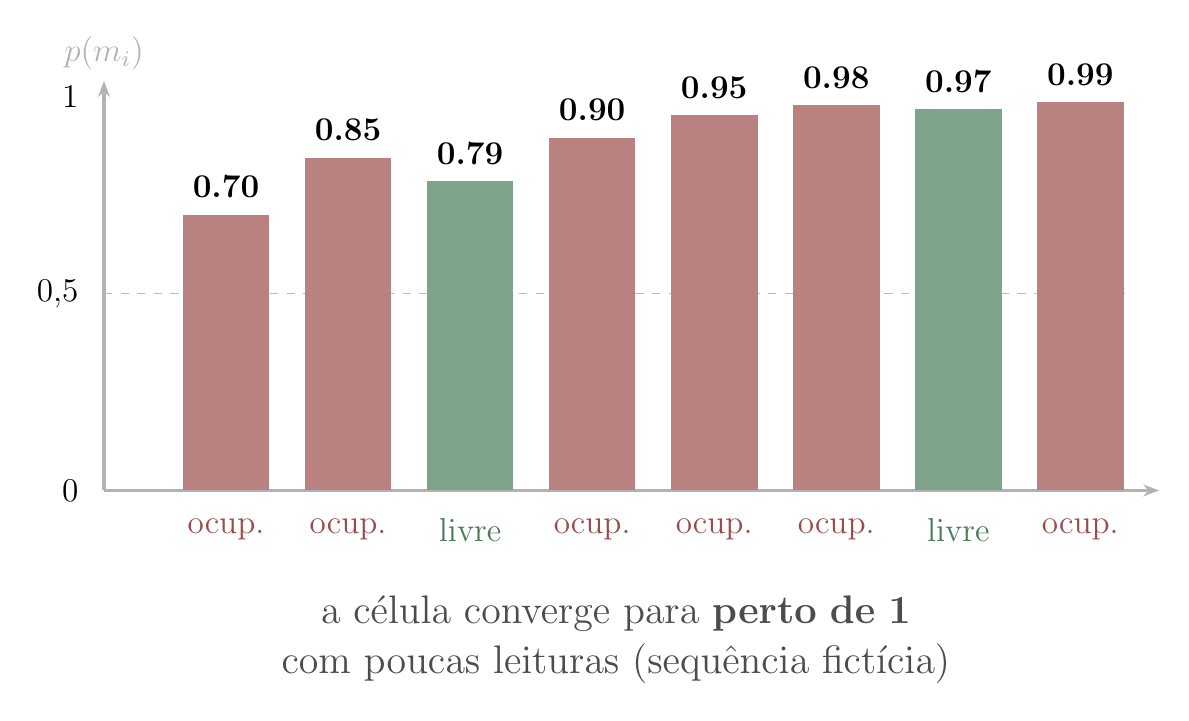
\begin{tikzpicture}[x=1cm,y=1cm]
  \pgfmathsetmacro{\lo}{0.85}\pgfmathsetmacro{\lf}{-0.4}
  \draw[daxis, line width=1.2pt] (0,0) -- (13.4,0); \draw[daxis, line width=1.2pt] (0,0) -- (0,5.2) node[above, font=\large] {$p(m_i)$};
  \draw[dguide] (0,2.5) -- (13.0,2.5); \node[font=\large, anchor=east] at (-0.2,2.5) {0,5}; \node[font=\large, anchor=east] at (-0.2,5.0) {1}; \node[font=\large, anchor=east] at (-0.2,0) {0};
  \fill[dred!70] (1.0,0) rectangle (2.1,3.503);
  \node[font=\large\bfseries] at (1.55,3.853) {0.70};
  \node[font=\large, dred] at (1.55,-0.5) {ocup.};
  \fill[dred!70] (2.55,0) rectangle (3.65,4.228);
  \node[font=\large\bfseries] at (3.1,4.578) {0.85};
  \node[font=\large, dred] at (3.1,-0.5) {ocup.};
  \fill[dgreen!70] (4.1,0) rectangle (5.2,3.929);
  \node[font=\large\bfseries] at (4.65,4.279) {0.79};
  \node[font=\large, dgreen] at (4.65,-0.5) {livre};
  \fill[dred!70] (5.65,0) rectangle (6.75,4.478);
  \node[font=\large\bfseries] at (6.2,4.828) {0.90};
  \node[font=\large, dred] at (6.2,-0.5) {ocup.};
  \fill[dred!70] (7.2,0) rectangle (8.3,4.763);
  \node[font=\large\bfseries] at (7.75,5.113) {0.95};
  \node[font=\large, dred] at (7.75,-0.5) {ocup.};
  \fill[dred!70] (8.75,0) rectangle (9.85,4.896);
  \node[font=\large\bfseries] at (9.3,5.246) {0.98};
  \node[font=\large, dred] at (9.3,-0.5) {ocup.};
  \fill[dgreen!70] (10.3,0) rectangle (11.4,4.846);
  \node[font=\large\bfseries] at (10.85,5.196) {0.97};
  \node[font=\large, dgreen] at (10.85,-0.5) {livre};
  \fill[dred!70] (11.85,0) rectangle (12.95,4.933);
  \node[font=\large\bfseries] at (12.4,5.283) {0.99};
  \node[font=\large, dred] at (12.4,-0.5) {ocup.};
  \node[font=\Large, black!70, text width=13cm, align=center] at (6.5,-1.9) {a célula converge para \textbf{perto de 1} com poucas leituras (sequência fictícia)};
\end{tikzpicture}
\end{document}
